\documentclass[11pt,english,french]{scrreprt}
\usepackage{lmodern}
\usepackage{babel}
\renewcommand{\familydefault}{\rmdefault}
\usepackage[T1]{fontenc}
\usepackage{ucs}
\usepackage[utf8x]{inputenc}
\usepackage[a4paper]{geometry}
\geometry{verbose,tmargin=2cm,bmargin=2cm,lmargin=2cm,rmargin=2cm,headheight=2cm,footskip=1cm}
\setlength{\parskip}{\smallskipamount}
\setlength{\parindent}{0pt}

\usepackage{amsthm}
\usepackage{booktabs}
\usepackage{amsmath}
\usepackage[unicode=true, pdfusetitle,
 bookmarks=true,bookmarksnumbered=false,bookmarksopen=false,
 breaklinks=false,pdfborder={0 0 1},backref=false,colorlinks=false]
 {hyperref}

\makeatletter
\usepackage{colortbl}
\usepackage{color}
\usepackage[dvipsnames]{xcolor}
\usepackage{wrapfig}
\usepackage{graphicx}
\usepackage{listings}
\usepackage[calcwidth]{titlesec}
\usepackage{fix-cm}
\usepackage{multicol}
\usepackage{verbatim}
\usepackage{moreverb}
\usepackage{nicefrac}
\usepackage{amssymb}
\usepackage{array}
\usepackage{tabularx}
\usepackage{subfig}
\usepackage[french,ruled,vlined]{algorithm2e}
\SetAlgoProcName{Procédure}{proc}

\theoremstyle{remark}
  \newtheorem*{rem*}{Remarque}
\theoremstyle{definition}
  \newtheorem*{defi}{Définition}
  \newtheorem{ques}{Question}[section]

\definecolor{MyDarkBlue}{rgb}{0,0.08,0.45}

\lstset{language=C,
	 	basicstyle=\small\ttfamily,
		keywordstyle=\small\ttfamily,
		identifierstyle=,
		commentstyle=\textcolor{OliveGreen},
		columns=fullflexible,
		stringstyle=\small\ttfamily,
		showstringspaces=false,numberstyle=\tiny, breaklines=false, tabsize=4}

\titleformat{\section}[hang]{\sffamily\bfseries}
 {\Large\thesection}{12pt}{\Large}[{\titlerule[0.5pt]}]

\def\thickhrulefill{\leavevmode \leaders \hrule height 1pt\hfill \kern \z@}
\renewcommand{\maketitle}{\begingroup%
    \let\footnotesize\small
    \let\footnoterule\relax
    \parindent \z@
    \reset@font
    \begin{flushleft}
      \huge \sffamily \bfseries\color{orange} \@title
    \end{flushleft}
    \hrule height 1pt
    \begin{flushright}
      \large\sffamily\color{MyDarkBlue}\@author
    \end{flushright}
  \endgroup%
  \setcounter{footnote}{0}%
}

\AtBeginDocument{
  \def\labelitemi{\normalfont\bfseries{--}}
}

\makeatletter
\renewcommand\thesection{\arabic{section}}
\@addtoreset{section}{chapter}
\makeatother

\makeatother
\begin{document}
	
\title{LI310 - Examen 2008\\
Lundi 15 décembre 2008}
\author{Benjamin BARON}

\maketitle

\section{Techniques de transmission} % (fold)

Signal porteur d'informations de fréquences strictement inférieures à 15 kHz.\\
Echantillon produit codé sur 16 bits (ie. $2^{16}$ niveaux de quantification).\\
Message numérique produit transmis en bande de base.

\begin{ques}
	Fréquence d'échantillonnage $f_e$ a utiliser pour minimiser le débit du message numérique produit à l'issue de l'opération de numérisation.
	
	Théorème d'échantillonnage de Shannon :\[f_e > 2f_{max}\]
	Application numérique ($f_{max} = 15$ kHz) :\[f_e > 2\times 15 = 30\;\textrm{kHz}\]
\end{ques}

\begin{ques}\label{ques:2}
	Capacité $C$ du canal de transmission pour permettre la transmission de ce message numérique.
	
	Puisque le signal transmis est échantillonné à une fréquence d'échantillonnage $f_e=30$ kHz, et que le signal numérique est composé d'échantillons codés sur $r = 16$ bits, alors le canal de transmission doit avoir une capacité $C=f_e\times r=30\,000\times 16=480$ kbit/s au minimum.
\end{ques}


\begin{ques}
	Câble de bande passante $[0,\,200\textrm{ kHz}]$.\\
	Rapport signal-à-bruit : $\nicefrac{S}{N}=18$ dB.
	
	D'après la loi de Shannon, la capacité maximale du canal considéré est exprimée par :\[C_{max}=B\log_2\left(1+\frac{P_S}{P_N}\right)\]
	Or \[\frac{P_S}{P_N}=10^{\frac{\nicefrac{S}{N}}{10}}= 10^{\frac{18}{10}}\approx 63,096\]
	Ainsi, on a :\[C_{max}=200.10^3\times \log_2(1+63,096)=4,81.10^7\;\textrm{bit/s}=48,1\;\textrm{Mbit/s}\]
	
	Puisque $C_{max}=48\,100\;\textrm{kbit/s}>C=480\;\textrm{kbit/s}$, alors la transmission est théoriquement possible sur ce canal.
\end{ques}

\begin{ques}
	Utilisation d'un code NRZ binaire ($M=2$) pour réaliser la transmission.
	
	D'après la loi de Nyquist :\[C \leqslant 2B\log_2(M) = 2\times 200.10^3\log_2(2) = 400\;\textrm{kbit/s}\]
	Or $C=480$ kbit/s, donc c'est impossible.
\end{ques}

\begin{ques}
	Utilisation d'un code NRZ-8 ($M=8$) pour réaliser la transmission.
	
	D'après la loi de Nyquist : \[C \leqslant 2B\log_2(M) = 2\times 200.10^3\log_2(8) = 1\,200\;\textrm{kbit/s} \leqslant C_{max}\]
	Or $C=480$ kbit/s, donc c'est possible.
\end{ques}

\begin{ques}
	La transmission à l'aide d'un signal NRZ-8 n'est pas optimale car avec celle-ci, on peut transmettre des messages à un débit maximal de $1\,200$ kbit/s (voir question précédente). Or on veut transmettre des messages à un débit de 480 kbit/s au minimum.
	
	On calcule alors une nouvelle valeur de $M$ de telle sorte que $M$ soit une puissance de 2 par la formule :
	\[M\geqslant 2^{\frac{D}{2B}} = 2^{\frac{480}{2\times 200}} = 2,297\]
	Ainsi, la modulation NRZ-4 est la plus adéquate.
	
	La liaison va alors fonctionner à un débit binaire de 480 kbit/s comme calculé à la question \ref{ques:2}.
\end{ques}

\section{Routage à état de liens} % (fold)

On considère le réseau suivant :
\begin{figure}[h]
	\center
	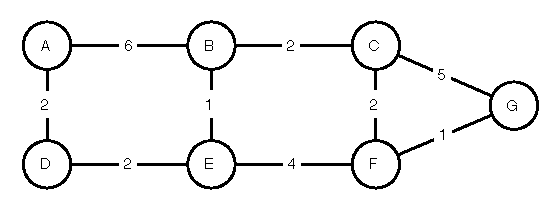
\includegraphics[scale=1]{Exam2009/graphe1}
\end{figure}

\begin{ques}
	Application de l'algorithme de Dijkstra pour le noeud A sur le réseau ci-dessus.\\
	Pour rappel, l'algorithme de Dijkstra est le suivant :\\
	\begin{algorithm}[H]
		\Donnees{$G=(S,\,A)$ un graphe orienté ; 
		$s$ : sommet racine de $G$ ; 
		$c\colon A\longrightarrow \mathbb{R}$ fonction coût sur les arcs telle que $\forall (x,\,y)\in A,\;c(x,\,y)\geqslant 0$}
		\DontPrintSemicolon
		\Deb{
			$d(s_1)\longleftarrow 0$\;
			\lstinline!ouvrir!($s_1$)\;
			\lPour{$k=2$ à $n$}{
				$d(s_k)\longleftarrow +\infty$\;
			}

			\Pour{$k=1$ à $n$}{
				$x\longleftarrow$ sommet ouvert tel que $d(x)$ minimum\;
				\PourTous{successeurs $y$ de $x$}{
					\Si{$d(y)>d(x)+c(x,\,y)$}{
						$d(y)\longleftarrow d(x)+c(x,\,y)$\;
						\lstinline!ouvrir!($y$)\;
					}
				}
				\lstinline!fermer!($s_k$)\;
			}
		}
		\caption{Algorithme de Dijkstra}
	\end{algorithm}
	
	Ordre de traitement des sommets : $A,\,D,\,E,\,B,\,C,\,F,\,G$.
	
	Arbre couvrant obtenu pour le noeud A : 
	\begin{figure}[h]
		\center
		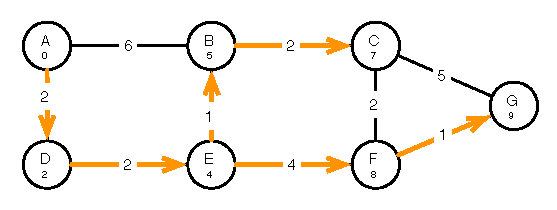
\includegraphics[scale=1]{Exam2009/graphe2}
	\end{figure}
\end{ques}

\begin{ques}
	Table de routage de A :\\
	\begin{tabularx}{\textwidth}{XXXX}
		\toprule 
		Destination & \emph{Next hop} & Chemin complet & Distance\tabularnewline
		\midrule
		\midrule 
		A & -- & -- & 0\tabularnewline
		\midrule 
		B & D & $A,\,D,\,E,\,B$  & 5\tabularnewline
		\midrule 
		C & D & $A,\,D,\,E,\,B,\,C$ & 7\tabularnewline
		\midrule 
		D & D & $A,\,D$ & 2\tabularnewline
		\midrule 
		E & D & $A,\,D,\,E$ & 4 \tabularnewline
		\midrule 
		F & D & $A,\,D,\,E,\,F$ & 8\tabularnewline
		\midrule 
		G & D & $A,\,D,\,E,\,F,\,G$ & 9 \tabularnewline
		\bottomrule
	\end{tabularx}
\end{ques}

\begin{ques}
	On suppose que les liens A-B, puis D-E, puis B-C tombent en panne. A chaque fois la machine (ou les machines) qui détecte la panne émet un LSP contenant une distance infinie pour le lien en question. 
	
	Représentation sous forme de graphe de la connaissance que A a du réseau une fois que tout est stabilisé (A n'a pas pu recevoir le LSP $(B,\,C,\,\infty)$) :
	\begin{figure}[h]
		\center
		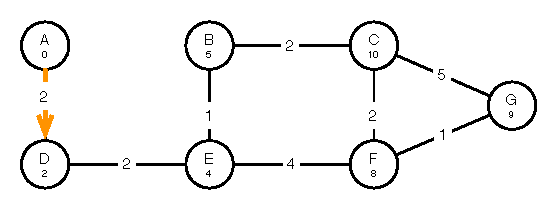
\includegraphics[scale=1]{Exam2009/graphe3}
	\end{figure}
\end{ques}

\begin{ques}
	Le lien D-E est rétabli, et le LSP correspondant est diffusé à tout le réseau.
	
	Arbre couvrant de A une fois que tout est stabilisé :
	\begin{figure}[h]
		\center
		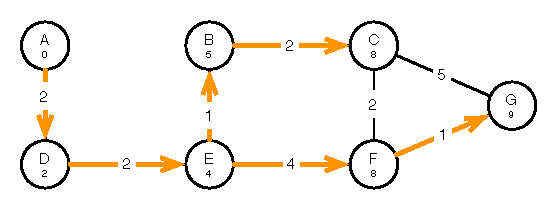
\includegraphics[scale=1]{Exam2009/graphe4}
	\end{figure}
	
	Table de routage de A :\\
	\begin{tabularx}{\textwidth}{XXXX}
		\toprule 
		Destination & \emph{Next hop} & Chemin complet & Distance\tabularnewline
		\midrule
		\midrule 
		A & -- & -- & 0\tabularnewline
		\midrule 
		B & D & $A,\,D,\,E,\,B$ & 5\tabularnewline
		\midrule 
		C & D & $A,\,D,\,E,\,B,\,C$ & 10\tabularnewline
		\midrule 
		D & D & $A,\,D$ & 2\tabularnewline
		\midrule 
		E & D & $A,\,D,\,E$ & 4 \tabularnewline
		\midrule 
		F & D & $A,\,E,\,F$ & 8\tabularnewline
		\midrule 
		G & D & $A,\,D,\,E,\,F,\,G$ & 9 \tabularnewline
		\bottomrule
	\end{tabularx}
\end{ques}

\begin{ques}
	Ce fonctionnement n'est pas satisfaisant car le lien B-C rompu n'a pas été pris en compte lorsque A a recalculé sa table de routage (le LSP correspondant n'avait été envoyé que sur le sous-graphe $\{B,\,C,\,E,\,F,\,G\}$).
	
	Pour palier à ce problème, il faut convenir d'une reprise après partitionnement du réseau. Les routeurs à chaque extrémité de la ligne rétablie vont coopérer pour restaurer les bases de données. Ils vont ainsi s'échanger les informations nécessaires, qui sont ensuite diffusées aux autres routeurs de leur partie de réseau.
\end{ques}

\section{Technique d'accès} % (fold)

Une des fonctionnalités de la couche liaison dans un environnement TCP/IP est de gérer l'accès au canal partagé. Pour cette raison, le protocole Ethernet implémente le mécanisme CSMA/CA (\emph{Carrier Sense Multiple Access with Collision Detection}) et bénéficie du fait que les stations peuvent écouter l'écho de leur transmission afin de détecter d'éventuelles collisions.

\begin{ques}
	Le principe du CSMA consiste à écouter le canal avant d'émettre. Si le coupleur détecte un signal sur le canal, il diffère son émission à une date ultérieure.
	
	Les collisions ne sont pas pour autant supprimées : Si, durant le temps de propagation entre le couple de stations les plus éloignées (période de vulnérabilité), un coupleur ne détecte pas l'émission d'une trame, il peut y avoir une superposition de signaux (et donc collision). De ce fait, il faut réémettre ultérieurement les trames perdues.
\end{ques}

Le mécanisme CSMA est aussi utilisé dans la couche liaison sans fil avec le protocole IEEE 802.11 (wifi). La spécificité du sans fil est que les stations ne peuvent pas émettre et écouter leur transmission en même temps. Afin d'éviter les collisions, le protocole IEEE 802.11 nécessite l'échange d'un total de 4 messages (3 messages de contrôle + 1 trame de données) pour envoyer une seule trame de données. Ce mécanisme est appelé CSMA/CA (\emph{Carrier Sense Multiple Access with Collision Avoidance}).

Considérons une trame de données à envoyer de taille 4504 octets, 3 autres messages de contrôle de 48 octets chacuns seront ajoutés.

\begin{ques}
	En supposant que le temps d'attente entre chacun des messages est de 1 ms et que le temps de propagation sur le support sans fil est négligeable, calculer au niveau liaison le temps nécessaire pour envoyer entièrement la trame. Supposez un lien sans fil de 2 Mbit/s.
	
	On a alors :\[\frac{504\times 8}{2.10^6}+3\times\frac{48\times 8}{2.10^{6}}+3\times1.10^{-3}=5,592\;\textrm{ms}\]
\end{ques}

Ping et délai.\\
Nous voulons dans cette partie comparer le délai aller-retour dans un réseau sans fil à ce même délai dans un réseau filaire. Dans les deux cas, nous allons négliger les temps de traitement et de propagation et ne considérer que le temps de transmission.

\begin{ques}
	Calculer le temps aller-retour d'un ping (\lstinline!echo request!, \lstinline!echo reply!) entre les machines A et B du réseau sans fil, sachant que la taille de la trame contenant le ping est de 104 octets et en gardant les mêmes hypothèses précédentes pour le réseau sans fil.
	
	Le délai aller-retour est alors exprimé par : \[2\times\left(\frac{104\times8}{2.10^6}+3\times\frac{48\times 8}{2.10^6}+3\times 1.10^{-3}\right)=7,984\;\textrm{ms}\]
\end{ques}

\begin{ques}
	Calculer le délai aller-retour si la technologie CSMA/CD (classique) est utilisée entre A et B. Dans ce cas, nous considérons des liens Ethernet de 10 Mbit/s et que le point d'accès est maintenant remplacé par un routeur dont le temps de traitement est négligeable. 
	
	Avec CSMA/CD, seule la trame de données est transmise (pas de trames de contrôle).\\
	Le délai aller-retour est exprimé par :\[2\times\frac{104\times 8}{10.10^6}=166,4\;\mu\textrm{s}\]
	
	On en conclut que la liaison Ethernet est beaucoup plus performante qu'une liaison sans fil avec une performance 10 fois supérieure.
\end{ques}

\begin{ques}
	Dans le réseau filaire seulement, si avant d'envoyer le ping, les informations concernant l'adresse physique ne sont pas connues pour A sur le premier tronçon de la connexion, A doit envoyer une requête ARP afin de connaître l'adresse MAC de B (si sur le même réseau local) ou celle du routeur qui se trouve sur le même réseau local que A.
\end{ques}

\section{Configuration IP} % (fold)

Dans une salle machine, vous vous loggez sur une machine UNIX. Une étiquette vous indique l'adresse IP de cette machine : 131.228.17.166.

\begin{ques}
	Cette adresse est une adresse de classe B car $131_d = 1000\,0011_b$ (préfixe 10).\\
	Masque par défaut associé à cette adresse de classe B : 255.255.0.0 
\end{ques}

\begin{ques}
	Adresse du réseau obtenue en faisant un ET logique entre le masque déterminé ci-dessus et l'adresse IP de la machine donnée. L'identifiant de la machine est obtenu en faisant un ET logique avec l'inverse du masque et l'adresse IP donnée.\begin{itemize}
		\item \emph{netid} : 131.228
		\item \emph{hostid} : 17.166
	\end{itemize}
\end{ques}

Vous souhaitez :\begin{itemize}
	\item vérifier que l'adresse IP indiquée sur l'étiquette est correcte ;
	\item connaître la valeur du masque utilisé ;
	\item connaître l'adresse de diffusion sur ce réseau
\end{itemize}

\begin{ques}
	La commande UNIX permettant d'obtenir ces trois informations est \lstinline!ifconfig -a! qui se trouve généralement à l'emplacement : \lstinline!/sbin/ifconfig!.
\end{ques}

Le résultat de cette commande ci-dessus vous indique que le masque utilisé est 255.255.255.240.

\begin{ques}
	A partir du masque par défaut (255.255.0.0), on calcule ne nombre maximum de sous-réseaux permet de créer cette subdivision.
	
	Le \emph{subnetid} est codé sur $8+4=12$ bits, donc il y a au maximum $2^{12}$ sous-réseaux créés par cette subdivision.
\end{ques}

\begin{ques}
	Adresse du réseau (\emph{subnetid}) sur lequel la machine est connectée. Il suffit de faire un ET logique entre l'adresse IP de la machine et le masque du sous-réseau donné.
	
	L'adresse du sous-réseau est alors : 131.228.17.160/28
\end{ques}

\begin{ques}
	L'identifiant de la machine (\emph{hostid}) s'obtient en faisant un ET logique entre l'adresse IP de la machine et le masque de sous-réseau.
	
	Identifiant de la machine sur ce réseau : 6
\end{ques}

\begin{ques}
	L'adresse de diffusion du sous-réseau est obtenue en faisant les opérations :\[(\textrm{Adresse}\;et\; \textrm{Masque})\;ou\; non \;(\textrm{Masque})\]
	Adresse de diffusion (\emph{broadcast}) sur ce réseau : 131.228.17.175/28
\end{ques}

La machine sur laquelle vous êtes connecté possède une seule carte réseau Ethernet. Pour accéder à Internet, les paquets passent par une passerelle.

\begin{ques}
	Nombre d'adresses IP possibles pour la passerelle. Cette passerelle est connectée au réseau local où se trouve la machine sur laquelle nous sommes loggé. De ce fait, il y a $2^4 - 2 = 14$ adresses IP différentes possibles pour la passerelle.
	
	Ce sont les adresses IP comprises entre 131.228.17.161/28 et 131.228.17.174/28.
\end{ques}

\begin{ques}
	On considère que la passerelle l'adresse 131.228.17.174/28. De plus, on considère que l'interface eth0 de la machine est la seule interface réseau à être connectée au réseau local.
	
	La table de routage minimale de la machine est alors :
	
	\begin{tabularx}{\textwidth}{XXXll}
		\toprule 
		Adresse & Masque & Prochain saut & Interface & Métrique\tabularnewline
		\midrule
		\midrule 
		131.228.17.174 & 255.255.255.240/28 & {*} & eth0 & 0\tabularnewline
		\midrule 
		default & 0.0.0.0 & 131.228.17.174 & eth0 & \tabularnewline
		\bottomrule
	\end{tabularx}
\end{ques}

\begin{ques}
	La table de routage de la machine peut être obtenue à l'aide de la commande \lstinline!route -n!
\end{ques}

\section{Codage / Décodage} % (fold)

On considère deux machines X et Y interconnectées via deux réseaux A et B et un routeur R.
% figure ici

Une trace a été obtenue sur le réseau A (Ethernet). De cette trame a été extraite la trame suivante (donnée sans préambule, ni CRC).

\begin{ques}
	Décodage de la trame :
	\begin{figure}[h]
		\center
		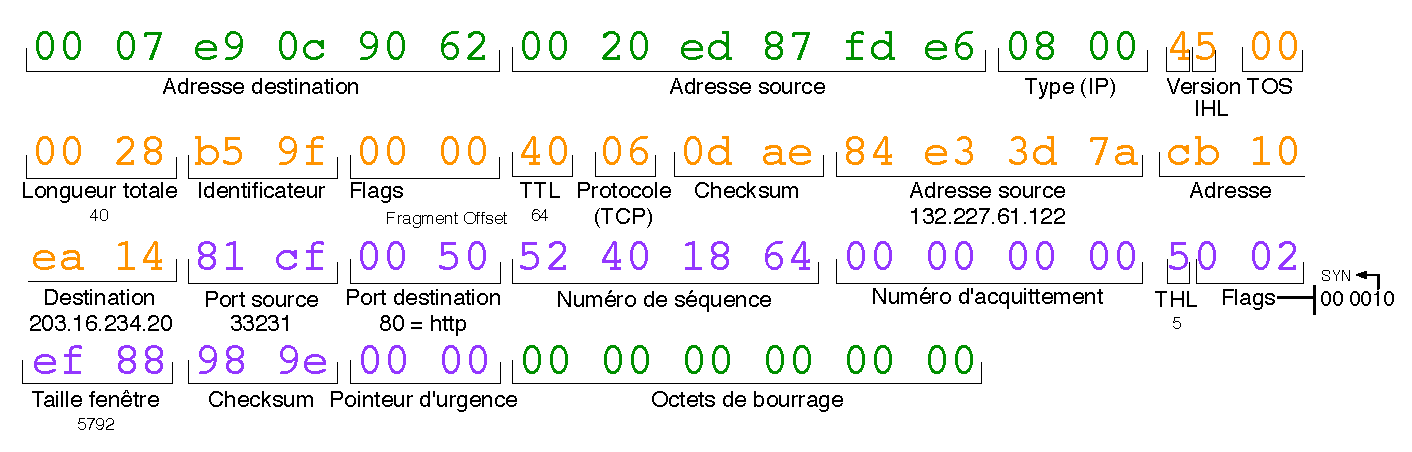
\includegraphics[scale=.7]{Exam2009/trame3}
	\end{figure}
	
	Protocoles utilisés au cours de la communication :\begin{itemize}
		\item Niveau Réseau : IP
		\item Niveau Transport : TCP 
		\item Niveau Application : http (port 80)
	\end{itemize}
	
	L'envoi de cette trame correspond à la demande d'établissement d'une requête TCP (flag \lstinline!SYN!) du client 132.227.61.122 au serveur 203.16.234.20. Le client a probablement lancé son navigateur qui a alors envoyé cette trame.
	
	Le champ \emph{data} d'une trame Ethernet doit comporter entre 46 et 1500 octets. De ce fait, les six derniers octets de cette trame correspondent à des octets de bourrage pour atteindre la valeur de 46 octets.
\end{ques}

\begin{ques}
	On suppose que le réseau B utilise un protocole d'accès dont la structure de trame est la même que celle d'Ethernet, à la différence que son champ de données ne peut excéder 36 octets de longueur.
	
	Suite à l'émission de la trame précédente sur le réseau A, deux trames seront ré-acheminées sur le réseau B :\begin{itemize}
		\item Le premier fragment contient un entête IP de 20 octets (Fragment offset = 0 et More Fragments = 1) et 16 octets de données ;
		\item Le second fragment contient un entête IP de 20 octets (Fragment Offset = 16/2 = 2 et More Fragments = 0) et le reste de données, soit 8 octets de données (dont 4 octets de bourrage). 
	\end{itemize}
	
	Les trames suivantes ont été transmises.
	\begin{figure}[h]
		\center
		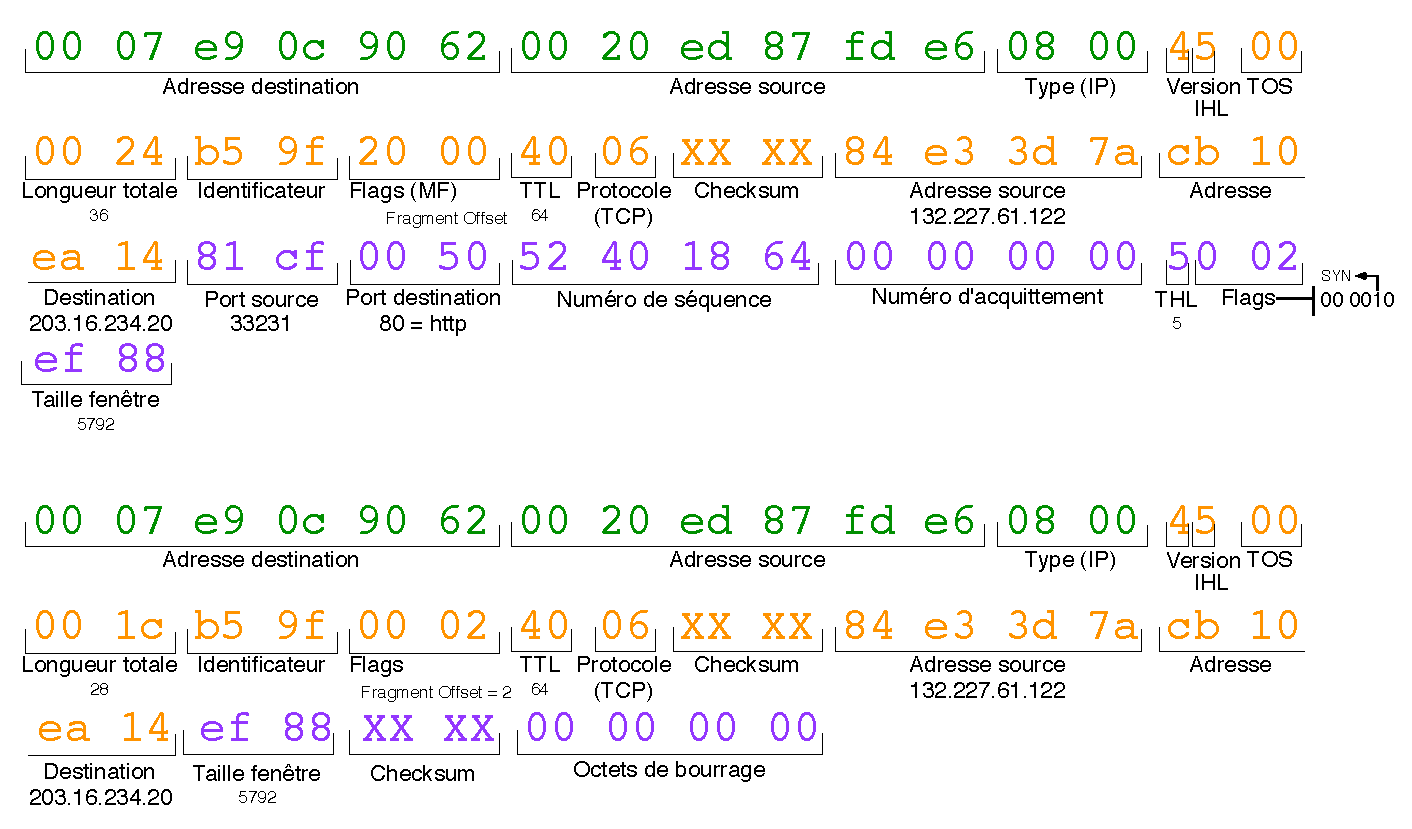
\includegraphics[scale=.7]{Exam2009/trame34}
	\end{figure}
\end{ques}
\end{document}